\chapter{Software Requirement Specification}

\section{Introduction}
\subsection{Purpose and Scope of Document}
Facilitating other Documentation: This SRS serves as a foundational reference for all future project documentation, including system design documents, test plans, user manuals, and project reports. It ensures consistency across development phases by providing a clear understanding of system requirements and expected behavior.

Product Validation: The SRS enables validation by establishing measurable criteria for evaluating the system's performance and verifying that the final implementation meets user requirements. It acts as a benchmark for acceptance testing to ensure the predicted geolocation results are accurate, reliable, and aligned with project objectives.

\subsection{Characteristics of a Software Requirement Specification}
Accuracy: The SRS clearly defines the functional and non-functional requirements without ambiguity. Every requirement accurately reflects the intended system behavior, such as input image handling, machine learning-based geolocation prediction, and result interpretation. Accurate details ensure developers and stakeholders share a common understanding.

Completeness: The SRS provides a complete description of all required system features, constraints, performance expectations, and interfaces. It includes functional requirements such as dataset processing, model training, and location prediction, as well as non-functional aspects like performance, security, usability, and scalability. No essential requirement is omitted.

Prioritization of Requirements: The requirements in the SRS are organized based on importance and implementation priority. Critical functionalities such as image preprocessing and model prediction are placed at higher priority, followed by enhancements like user interface improvements, accuracy tuning, and dataset expansion. Prioritization ensures efficient planning and phased development.

\subsection{Overview of Responsibilities of Developer}
The development responsibilities include frontend design, backend API implementation, multimodal model integration, database schema design, validation logic, safety policy implementation, and testing. The developer must ensure that the system does not perform automatic authority dispatch and that all report actions are explicitly confirmed by the user.

\section{Usage Scenario}
The system is designed for users who want to understand an image, identify possible place context, or receive safety-aware guidance. A user opens the web application, uploads an image, and submits it for analysis. The backend sends the image and prompt to the multimodal model, validates the returned JSON, applies policy rules, saves logs, and returns a response with actions.

\subsection{User Profiles}
\begin{table}[H]
\centering
\caption{System Entities Description}
\label{tab:entities}
\def\arraystretch{1.5}
\begin{tabularx}{\textwidth}{|c|l|X|}
\hline
\textbf{Sr. No.} & \textbf{Actor} & \textbf{Description} \\ \hline
1 & General User & Uploads an image and receives scene explanation, location estimate, risk level, and actions. \\ \hline
2 & Public Safety Observer & Uses the report flow when a hazardous or suspicious image is detected and confirms incident logging. \\ \hline
3 & Reviewer / Evaluator & Reviews stored model outputs, actions, confidence values, and incident records for project evaluation. \\ \hline
4 & System Administrator & Configures API keys, database path, upload size, and optional WhatsApp notification settings. \\ \hline
\end{tabularx}
\end{table}

\subsection{Use Cases}
\begin{table}[H]
\centering
\caption{Use Cases}
\label{tab:usecases}
\def\arraystretch{1.4}
\begin{tabularx}{\textwidth}{|c|X|X|c|X|}
\hline
\textbf{Sr. No.} & \textbf{Use Case} & \textbf{Description} & \textbf{Actors} & \textbf{Assumption}\\ \hline
1 & Analyze Image & User uploads an image and receives a structured scene interpretation. & User & Image format is supported. \\ \hline
2 & Learn More & User selects learn-more action for a normal landmark or place. & User & Place/entity is detected. \\ \hline
3 & Open Map & User opens a map search for the detected location. & User & Location guess is available. \\ \hline
4 & View Explanation & User checks why a result was produced. & User & Rationale is returned or fallback rationale exists. \\ \hline
5 & Report Suspicious Activity & User confirms incident reporting for high-risk output. & User & Confirmation is required before logging. \\ \hline
6 & Review Logs & Evaluator checks sessions, actions, and incidents. & Reviewer & Database records are available. \\ \hline
\end{tabularx}
\end{table}

\subsection{Use Case View}
The use case view represents interaction between users and the multimodal assistant. The primary user uploads an image and receives analysis. Based on the response, the user may learn more, open a map, view rationale, or confirm a report. The reviewer interacts with logs for evaluation.

\begin{figure}[H]
\centering
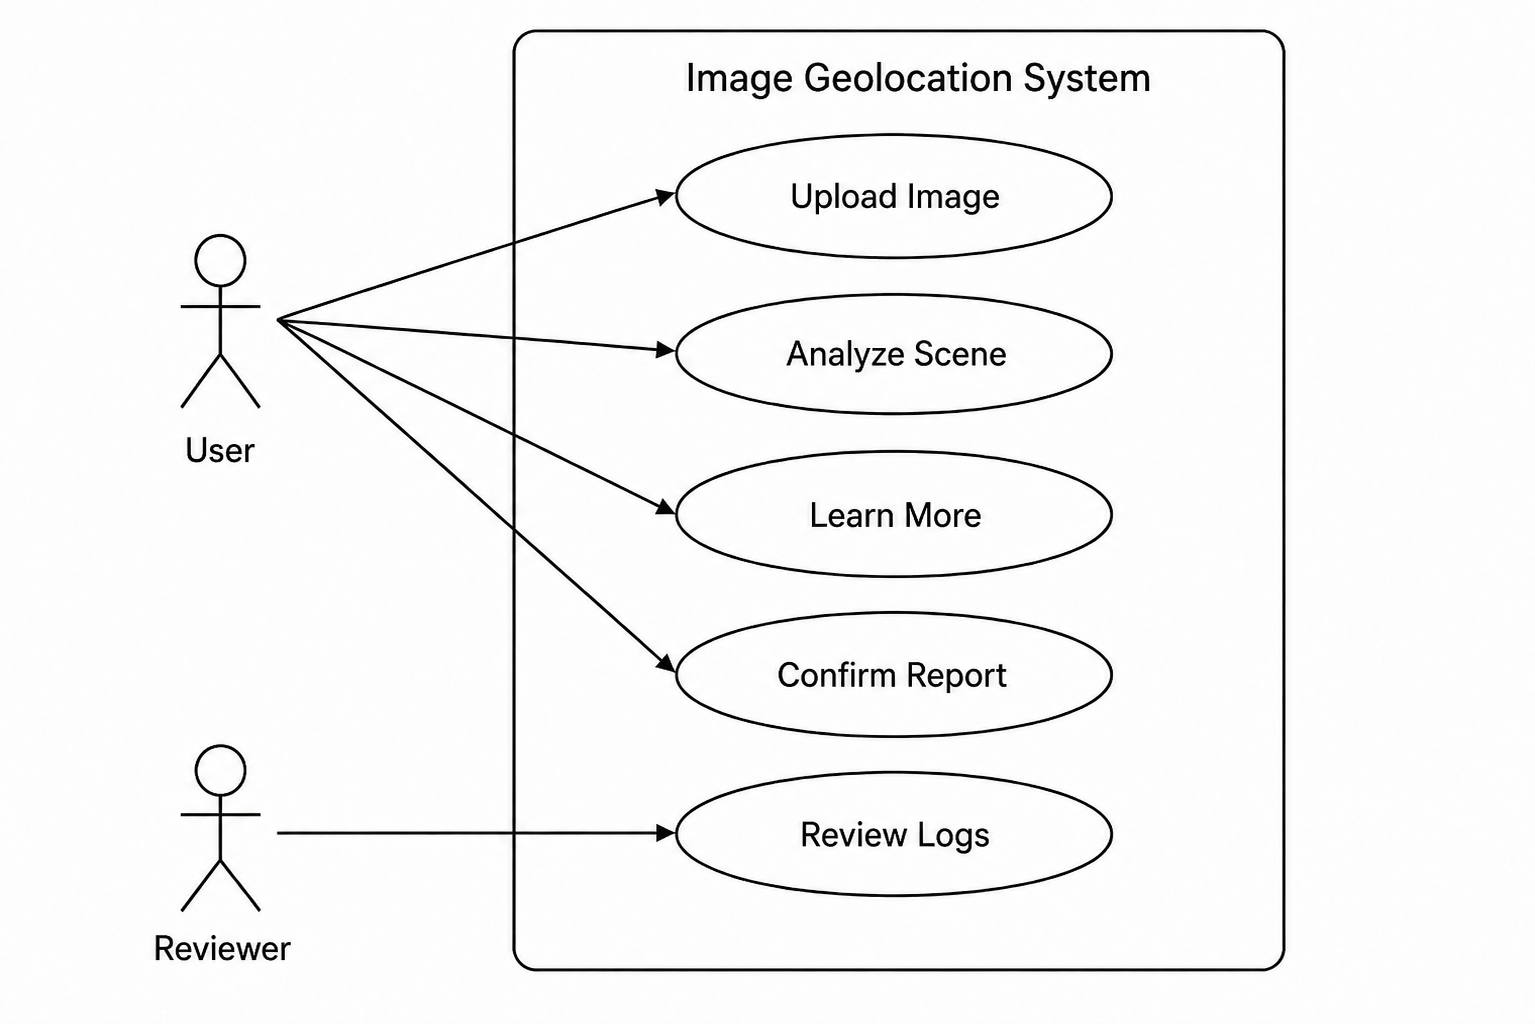
\includegraphics[width=0.95\textwidth]{diagrams/use-case.png}
\caption{Use case diagram}
\label{fig:usecase}
\end{figure}

\section{Data Model and Description}
\subsection{Data Description}
The system uses SQLite as the persistence layer. It stores session data, messages, structured model outputs, user actions, and incident records. Raw images are not stored by default; an image hash is saved for traceability and privacy.

\subsection{Data Objects and Relationships}
The main database tables are:
\begin{itemize}
\item \textbf{sessions}: Stores conversation sessions.
\item \textbf{messages}: Stores user and assistant messages with optional image hash.
\item \textbf{model\_outputs}: Stores risk level, confidence, and full JSON payload.
\item \textbf{actions}: Stores user-selected actions such as learn-more and report.
\item \textbf{incidents}: Stores user-confirmed incident reports and optional notification status.
\end{itemize}

\begin{figure}[H]
\centering
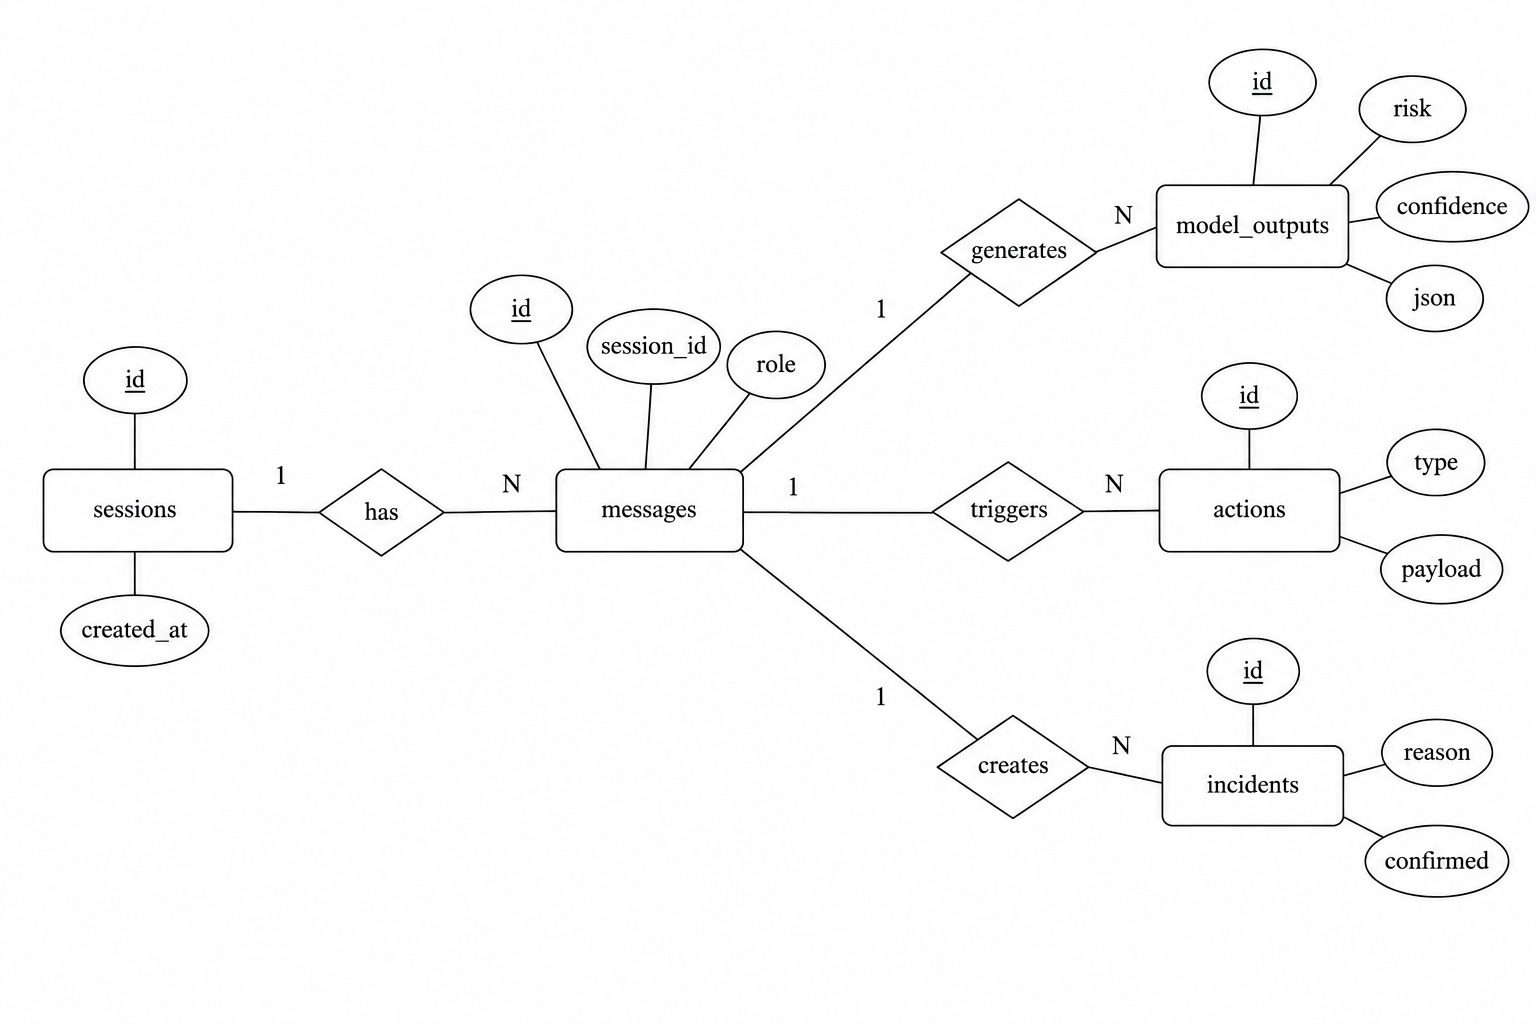
\includegraphics[width=0.95\textwidth]{diagrams/er-diagram.jpeg}
\caption{ER diagram}
\label{fig:er}
\end{figure}

\section{Functional Model and Description}
\subsection{Data Flow Diagram}
The data flow starts when a user submits an image. The frontend sends a multipart request to the backend. The backend validates input, hashes the image, invokes Gemini Vision, parses the model response, applies policy rules, saves records, and returns a response to the frontend.

\subsubsection{Level 0 Data Flow Diagram}
\begin{figure}[H]
\centering
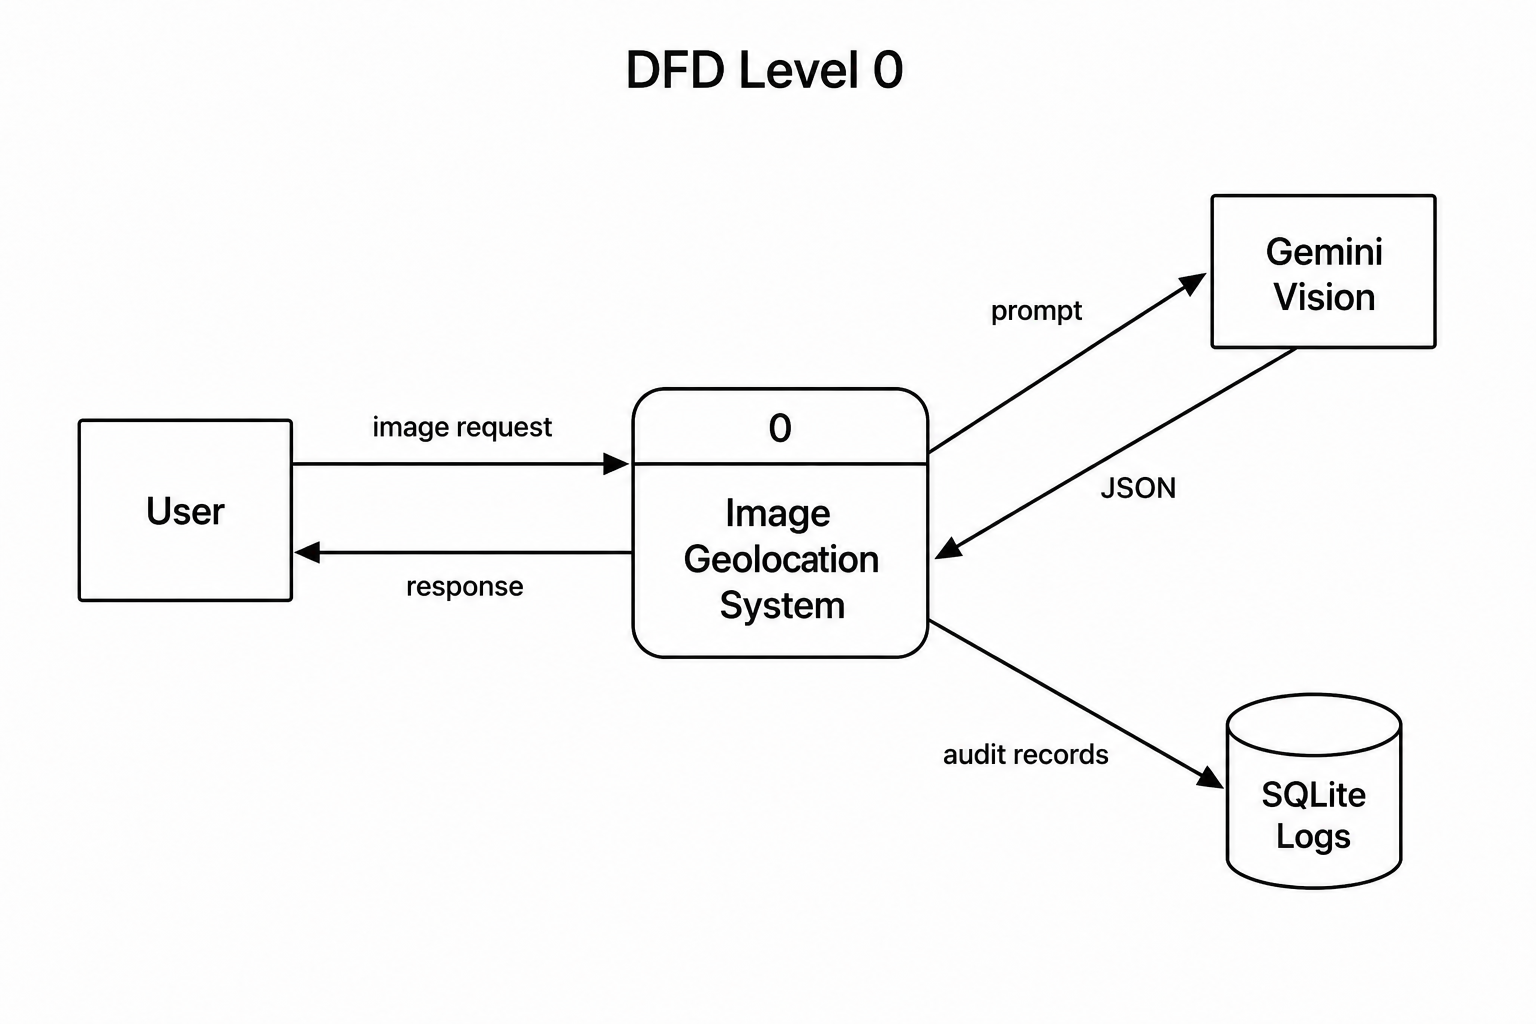
\includegraphics[width=0.95\textwidth]{diagrams/dfd-lvl-0.png}
\caption{DFD Level 0 diagram}
\label{fig:dfd0}
\end{figure}

\subsubsection{Level 1 Data Flow Diagram}
\begin{figure}[H]
\centering
\resizebox{0.92\textwidth}{!}{%
\begin{tikzpicture}[
process/.style={rectangle, draw, rounded corners, minimum width=32mm, minimum height=12mm, align=center, font=\small},
store/.style={cylinder, draw, shape border rotate=90, aspect=0.25, minimum height=15mm, minimum width=20mm, align=center, font=\small},
flow/.style={->, thick, shorten >=2pt, shorten <=2pt}
]
\node[process] (upload) at (0,0) {1. Upload\\Image};
\node[process] (infer) at (4.4,0) {2. Gemini\\Inference};
\node[process] (policy) at (8.8,0) {3. Risk Policy\\and Actions};
\node[process] (reply) at (13.2,0) {4. Response\\to User};
\node[store] (db) at (8.8,-2.6) {SQLite\\DB};
\draw[flow] (upload) -- (infer);
\draw[flow] (infer) -- (policy);
\draw[flow] (policy) -- (reply);
\draw[flow] (upload) |- (db);
\draw[flow] (policy) -- (db);
\draw[flow] (db) -- (reply);
\end{tikzpicture}
}
\caption{DFD Level 1 diagram}
\label{fig:dfd1}
\end{figure}

\subsection{Description of Functions}
The major functions of the system are image upload, model inference, JSON extraction, JSON repair, output normalization, hazard signal detection, action generation, learn-more lookup, map link generation, incident reporting, and audit logging.

\subsection{Activity Diagram}
The activity diagram represents the end-to-end workflow from image upload to action selection.

\begin{figure}[H]
\centering
\begin{tikzpicture}[
activity/.style={rectangle, draw, rounded corners, minimum width=46mm, minimum height=10mm, align=center, font=\small},
decision/.style={diamond, draw, aspect=2, align=center, inner sep=2mm, font=\small},
flow/.style={->, thick, shorten >=2pt, shorten <=2pt}
]
\node[circle, fill=black, minimum size=4mm] (start) at (0,0) {};
\node[activity] (upload) at (0,-1.2) {Upload image};
\node[activity] (analyze) at (0,-2.5) {Analyze with Gemini Vision};
\node[activity] (normalize) at (0,-3.8) {Validate and normalize JSON};
\node[decision] (risk) at (0,-5.3) {Risk\\high?};
\node[activity] (report) at (-3.6,-7) {Show report and\\safety actions};
\node[activity] (learn) at (3.6,-7) {Show learn-more\\and map actions};
\node[activity] (persist) at (0,-8.5) {Persist logs\\and actions};
\node[circle, draw, thick, minimum size=5mm] (end) at (0,-9.8) {};
\node[circle, fill=black, minimum size=3mm] at (0,-9.8) {};
\draw[flow] (start) -- (upload);
\draw[flow] (upload) -- (analyze);
\draw[flow] (analyze) -- (normalize);
\draw[flow] (normalize) -- (risk);
\draw[flow] (risk) -- node[above, sloped, font=\footnotesize]{yes} (report);
\draw[flow] (risk) -- node[above, sloped, font=\footnotesize]{no} (learn);
\draw[flow] (report) |- (persist);
\draw[flow] (learn) |- (persist);
\draw[flow] (persist) -- (end);
\end{tikzpicture}
\caption{Activity diagram}
\label{fig:activity}
\end{figure}

\subsection{Non Functional Requirements}
\begin{itemize}
\item \textbf{Performance}: The MVP targets response latency below 8 seconds for common demo cases.
\item \textbf{Reliability}: Invalid model output must trigger repair or safe fallback.
\item \textbf{Security}: API keys must be stored in environment variables and not logged.
\item \textbf{Privacy}: Raw images are not stored by default; image hashes are persisted.
\item \textbf{Usability}: The interface must show image preview, chat messages, and inline action buttons.
\item \textbf{Auditability}: Every model output, action, and incident must be stored for review.
\end{itemize}

\subsection{State Diagram}
The system state changes from image selection to analysis, output generation, action rendering, and optional incident creation.

\begin{figure}[H]
\centering
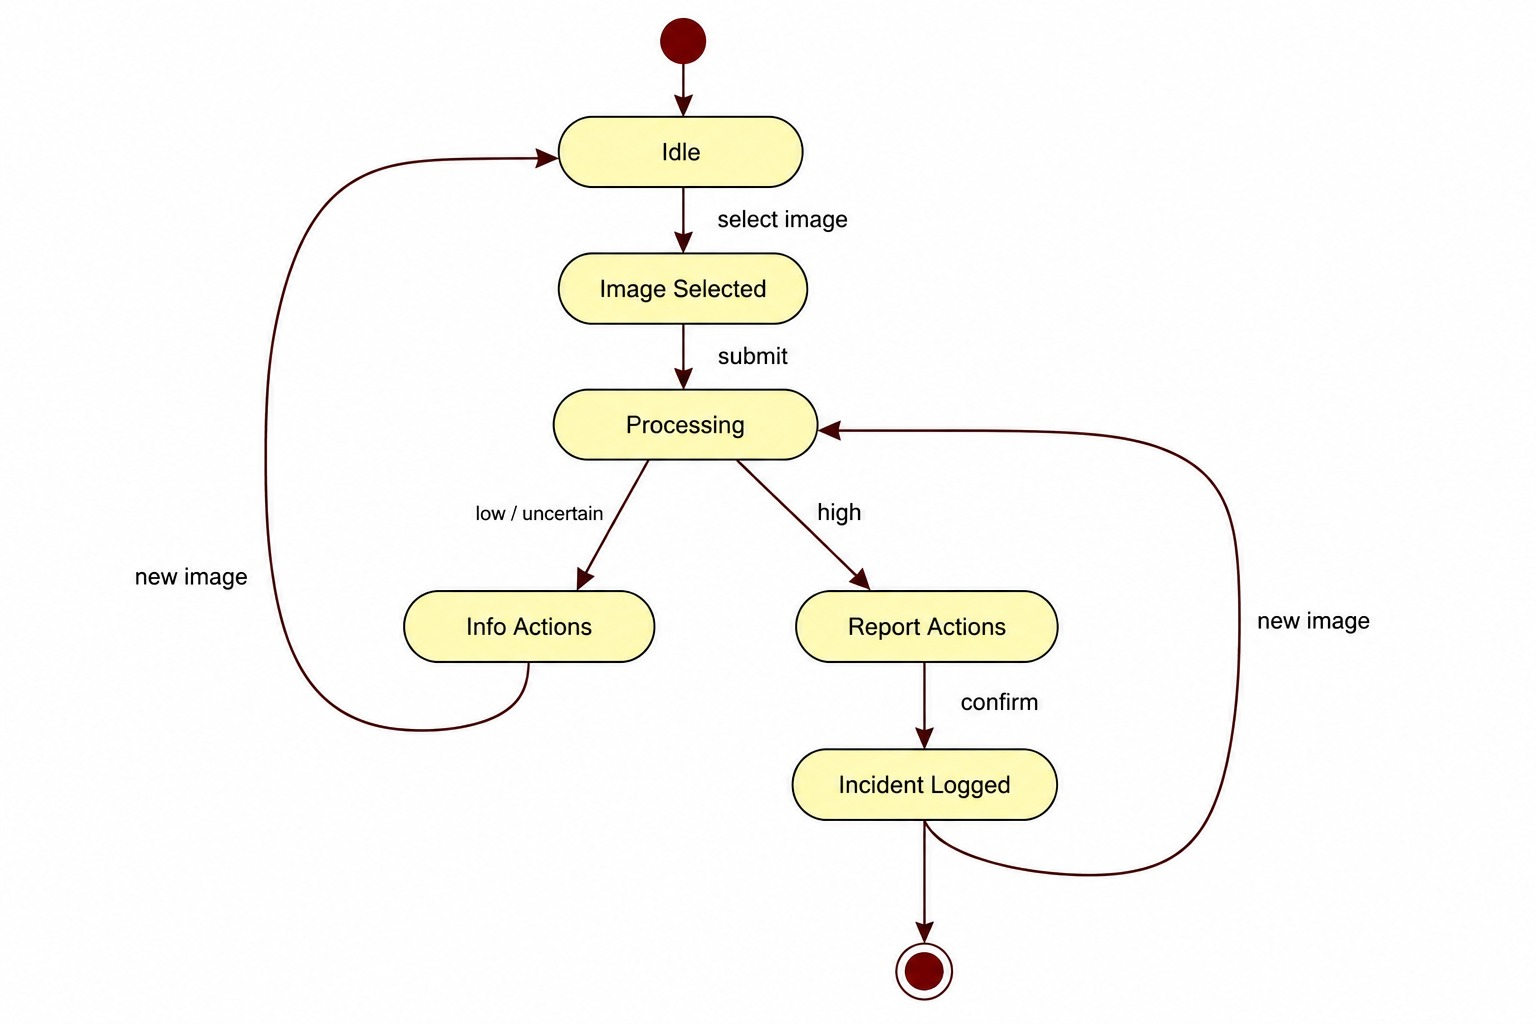
\includegraphics[width=0.95\textwidth]{diagrams/state-transition.jpeg}
\caption{State transition diagram}
\label{fig:state}
\end{figure}

\subsection{Design Constraints}
The system must not perform automatic external authority dispatch. WhatsApp notification is optional, environment-gated, and requires explicit user confirmation. The model must return strict JSON where possible, and fallback behavior must be conservative when confidence is low or output is invalid.

\subsection{Software Interface Description}
The backend exposes REST APIs for analysis, learn-more, report, and health check. The frontend communicates with these APIs using HTTP requests. Gemini Vision is accessed through the Google Generative Language API. Wikipedia is used for learn-more summaries, and Google Maps search links are generated for detected locations.
